\chapter{插图}\label{sec:graphics}

\begin{quotation}
A picture says more than a thousand words.
\begin{flushright}
--- Shakespeare
\end{flushright}
\end{quotation}

当年Knuth开发 \TeX 时,GIF、JPEG、PNG、EPS等图形格式还没有问世,所以DVI不能直接支持这些格式。但是高手就是高手,Knuth在 \TeX 里留了一个后门:\verb|\special| 命令,让后面的驱动自行决定怎样处理图形。

这和当年老毛把港澳台,老邓把钓鱼岛都“留给后人解决”有异曲同工之妙。曾经有位出版社的编辑看上了包老师写的一个程序,要我改改当作教学辅助软件出版,但是当时手头没有DOS中断的资料没办法加鼠标操作。该编辑说:你把鼠标驱动打包在软件里,让用户自己琢磨是怎么回事。

下面我们会在 \ref{sec:graphics_format} 节讨论 \LaTeX 所用图形格式以及图形的优化、转换和处理,\ref{sec:includegraphics} 节介绍怎样插入图形,\ref{sec:draft} 节简介矢量绘图。接下来的六至八章会分别讨论怎样使用 \MP, PSTricks和PGF。

\section{图形概览}
\label{sec:graphics_format}

\subsection{图形格式}

\LaTeX 支持点阵图形格式JPEG和PNG,也支持矢量格式EPS和PDF \footnote{EPS和PDF中也可以嵌入点阵图形,但是它们本身还是矢量格式。}。对于示意图,我们应该首选矢量格式;包含大量自然色彩的图像 (比如照片) 应该选JPEG;人工点阵图像应该选PNG。

1980年代中后期,PostScript风头之劲一时无两,人们自然会考虑把它作为文档中嵌入图形的标准格式。然而它实在太强大,人们担心嵌入文档的PostScript会搞破坏,于是就产生了戴着手铐的Encapsulated PostScript (EPS) 。出于同样的原因,人们也担心嵌入HTML的ActiveX、Java Applet、JavaScript中混入恶意代码,所以才会对它们也有所限制。早年间人们得到DVI后通常会把它转换为PostScript,所以EPS就成了 \LaTeX 的标准图形格式。
 
\subsection{Driver的口味}

\subsubsection{dvips}

\texttt{dvips} 喜欢PostScript,所以就爱屋及乌只支持嵌入EPS。MiKTeX看不惯这种垄断行为,就把 \texttt{dvips} 破解,添加了对JPEG和PNG的支持。但是它很固执,坚持按缺省分辨率72 PPI计算图形尺寸,并认为所有图形都是灰度图。为了避免麻烦,包老师还是劝你把这些图形格式转换为EPS。

\subsubsection{pdflatex}
\texttt{pdflatex} \footnote{\texttt{pdflatex} 包含编译和驱动两种功能,所以这里也就把它划到驱动一边。} 支持JPEG、PNG和PDF,不支持EPS。传说它不支持EPS的原因是PostScript解释器的版权问题。包老师认为这种说法不可信,因为1997年pdfTeX面世时PostScript已经被PDF赶超,Adobe与其保护PostScript还不如保护PDF。

\LaTeX 有两个宏包 \texttt{epstopdf} 和 \texttt{pst-pdf} 可以实时地 (on the fly) 把EPS转换为PDF \footnote{在这里on the fly是指在后台处理,用户不用操心。包老师不确定把它翻译为“实时”是否合适,因为real time通常被翻译为实时。对于用户无须干涉、知情的情况,有人说user transparent,也有人说black box,语言还真奇妙。}。然而前者有安全漏洞,后者用法繁琐,用户最好还是用其他软件事先把EPS转为PDF。

\subsubsection{dvipdfm(x)}

\texttt{dvipdfm} 支持JPEG、PNG和PDF,不支持EPS,但是它可以实时地调用Ghostscript把EPS转为PDF。\texttt{dvipdfmx} 对上述图形格式的支持有所增强,还增加了对BMP的支持。

\subsubsection{xdvipdfmx}

\XeLaTeX 的缺省驱动 \texttt{xdvipdfmx} 直接支持BMP、JPEG、PNG、EPS和PDF。所以从图形格式支持的角度来讲,\texttt{xdvipdfmx} 比 \texttt{dvips、pdflatex} 和 \texttt{dvipdfmx} 都好。传说 \texttt{xdv2pdf} 驱动还支持GIF、PICT、PSD、SGA、TGA、TIFF等格式,可惜只能在Mac OS X上用。

\subsection{图形优化}

矢量图形的一个优点是可以无限缩放,而输出质量不变。图形尺寸对矢量图形而言意义不大。描述矢量图形所需数据较少,所以其文件体积一般也较小。

而点阵图形是以像素 (pixel) 为单位描述、存储的,图形尺寸越大,文件体积就越大。当然影响文件体积的还有色彩深度、压缩算法等因素。

人们一般希望用较小的文件体积获取较好的输出效果,这样就需要优化图形尺寸和色彩。

\subsubsection{图形尺寸}

点阵图形的像素是一种相对尺寸,其实际尺寸等于像素除以分辨率 (resolution) ,最常用的分辨率单位是像素/英寸 (pixels per inch,PPI) 。在古时候PPI也常和点/英寸 (dots per inch, DPI) 混用;现在人们倾向于认为PPI是图形的分辨率单位,而DPI是硬件设备 (比如显示器或打印机) 输出的分辨率单位。通常横向和纵向分辨率相同,可以写成一个数字。

比如有一幅100 x 150像素的点阵图形 (\autoref{fig:default_size}) ,其分辨率为100 PPI。在输出时,它的缺省尺寸就是1in x 1.5in。如果我们将它强制输出为2in x 3in (\autoref{fig:force_size}) ,那么其实际分辨率就降为50 PPI。

\begin{figure}[htbp]
\centering
\begin{minipage}[b]{1.4in}
\centering
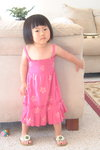
\includegraphics{anna.jpg}
\caption{缺省输出尺寸}
\label{fig:default_size}
\end{minipage}
\hspace{10pt}
\begin{minipage}[b]{2in}
\centering
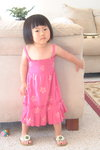
\includegraphics[width=2in]{anna.jpg}
\caption{强制放大输出尺寸}
\label{fig:force_size}
\end{minipage}
\end{figure}

假设输出分辨率是100 DPI,像素和输出点就一一对应;如果输出分辨率是300 DPI,每个像素实际输出为3 x 3个点;如果输出分辨率是50 DPI,每2 x 2个像素才享受到一个输出点的待遇。

当图形分辨率和输出分辨率不一致时,就会有一个重新采样 (resampling) 的过程;从高分辨率到低分辨率叫下采样 (downsampling) ,反之叫上采样 (upsampling) 。重新采样的插值 (interpolation) 算法有很多,其中常用的有最近像素 (nearest neighbor) 、双线性 (bilinear) 、双三次 (bicubic) 、兰索斯 (Lanczos) 等。前两种速度快,但是效果差;后两种效果好,但是速度慢。追求完美的雷人自然要选择Lanczos。

一般而言,高分辨率图形配合高分辨率输出设备会产生高质量效果,低分辨率图形配合低分辨率设备会产生低质量效果;高分辨率图形遇到低分辨率设备会形成浪费;低分辨率图形遇到高分辨率设备呢,得看插值效果,但是最好嫑高估机器的智能。雷人追求的是高质量文档,所以输出设备的分辨率大家暂时就甭操心了。

当输出尺寸一定时,图形分辨率越高需要的像素就越多,图形文件体积就越大。那么点阵图形的分辨率多少比较合适呢?一般认为在屏幕上阅读需要72 PPI,考虑到放大150 PPI应该够了,而高质量打印需要300 PPI。

假设我们要在 \LaTeX 文档中嵌入一幅图形,如果是通栏,宽度就是4.8--5.4in (文档缺省宽度取决于字体大小) 。那么如果仅用于屏幕阅读,原始图形的宽度400px足够了;如要放大阅读或输出打印则分别需要800px和1600px。

点阵图形尺寸相关的基本编辑操作有以下几种:裁剪 (crop) 、改尺寸 (resize) 、改分辨率。

\begin{enumerate}
\item 裁剪时像素自然会变少,分辨率不变,缺省输出尺寸也就变小。\autoref{fig:default_size} 其实就是从一幅2048 x 1536像素的大图裁剪、缩小而来,因为原图太大,\autoref{fig:original} 把它强制输出为4in x 3in。

\item 改尺寸时像素改变,分辨率不变,缺省输出尺寸相应改变,这个过程需要重新采样。比如把 \autoref{fig:default_size} resize到200 x 300像素,分辨率还是100 PPI,那么缺省输出尺寸就变成2in x 3in (\autoref{fig:resize}) 。

\item 单纯更改图形文件分辨率时,像素不变,缺省输出尺寸相应改变。把 \autoref{fig:default_size} 分辨率设为200 PPI,像素还是100 x 150,那么缺省输出尺寸就变成0.5 x 0.75in (\autoref{fig:density}) 。

\item 改尺寸和改分辨率可以结合使用。把 \autoref{fig:default_size} 的尺寸改为200 x 300像素,分辨率改为200 PPI,缺省输出尺寸就还是1in x 1.5in (\autoref{fig:resample}) 。
\end{enumerate}

综上所述,点阵图形的信息量取决于像素。图形文件的分辨率只是“建议”缺省输出尺寸,并不影响图形质量。上述操作中裁剪和改尺寸比较实用,改分辨率没有实质意义。改尺寸一般也只能从大改小。如果从小改大的话,插补出来的像素比起原装的还是要差一些。

\begin{figure}[htbp]
\centering
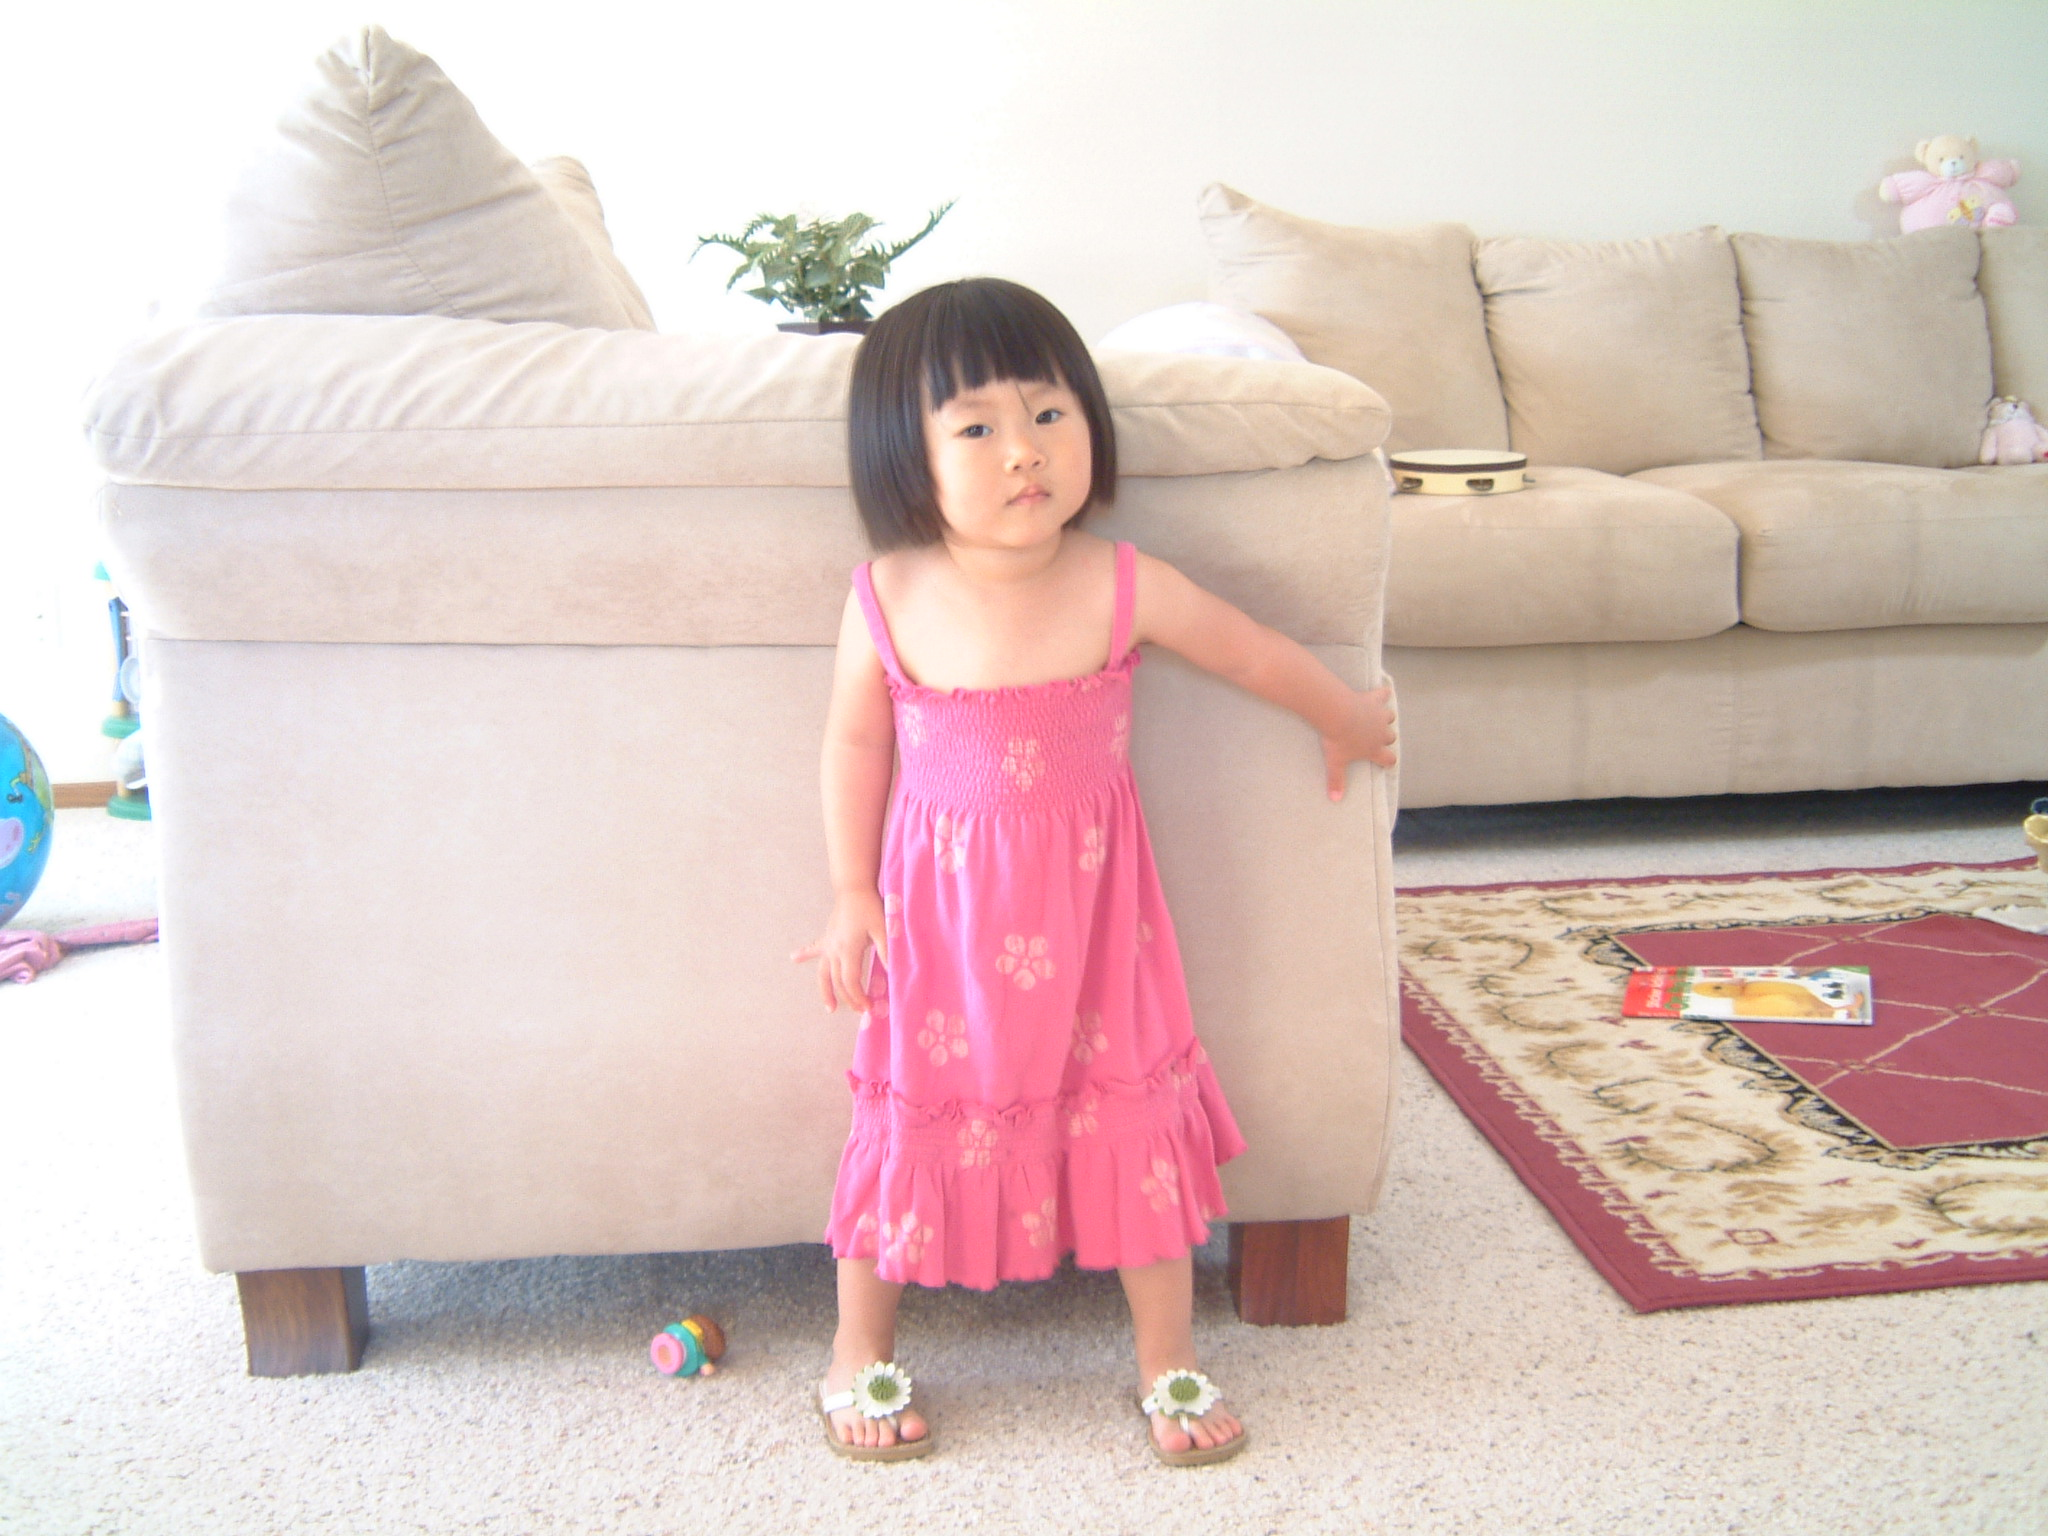
\includegraphics[width=4in]{dscf6030.jpg}
\caption{原始图形}
\label{fig:original}
\end{figure}

\begin{figure}[!htbp]
\centering
\begin{minipage}[b]{2in}
\centering
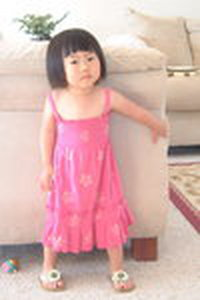
\includegraphics{anna_resize.jpg}
\caption{改尺寸}
\label{fig:resize}
\end{minipage}
%\hspace{5pt}
\begin{minipage}[b]{1.1in}
\centering
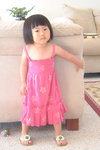
\includegraphics{anna_density.jpg}
\caption{改分辨率}
\label{fig:density}
\end{minipage}
%\hspace{5pt}
\begin{minipage}[b]{1.6in}
\centering
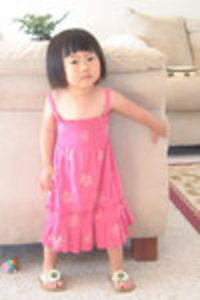
\includegraphics{anna_resample.jpg}
\caption{改尺寸和分辨率}
\label{fig:resample}
\end{minipage}
\end{figure}

需要指出的是上述操作在不同的软件里名称不同,比如改尺寸,相当于ImageMagick中的resize和Adobe PhotoShop中的resample;改分辨率,相当于ImageMagick中的density和PhotoShop中的resize;上面第四种混合操作,在ImageMagick叫resample。包子曰:道可道,非常道。名可名,非常名。

\subsubsection{色彩深度}

色彩深度 (color depth) 是每一个像素所用颜色的位数。比如一位可以表示两种颜色,通常是黑白;两位可以表示四色,最早用于CGA显卡;四位16色,用于EGA显卡;八位256色,用于VGA显卡;16位65,536色,又称高彩;24位16,777,216色,又称真彩;30--48位称为深彩。

色深位数越高越逼真,文件体积也就越大。一般照片可以用24位,人工图像用八位足矣,图标之类的小图形可以考虑更少位数。从 \autoref{fig:depth} 我们可以看到各种色深的效果和文件体积,它们都是PNG格式。

\begin{figure}[htbp]
\centering
\begin{tabular}{ccc}
    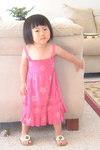
\includegraphics{anna.png} & 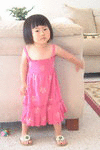
\includegraphics{anna8.png} &  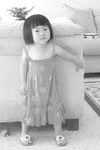
\includegraphics{anna8g.png} \\
    24位真彩 34 KB & 8位256色 23.4 KB & 8位灰度 18.7 KB \\
    
\includegraphics{anna4.png} & 
\includegraphics{anna2.png} &  
\includegraphics{anna1.png} \rule{0pt}{111pt} \\
    4位16色 15.6 KB & 2位4色 13.5 KB & 1位黑白 12 KB
\end{tabular}
\caption{色彩深度}
\label{fig:depth}
\end{figure}

我们一般也只能把图形的色深从高改低,从而减小图形文件和最终文档的体积。反过来把低色深从低改高,属于逆势而为,或遭天谴。

\subsection{图形转换和处理}

按说有了 \XeLaTeX 之后雷人已经基本上不再需要转换图形格式,只是有时出版社会指定使用某几种图形格式;另外我们常常需要优化图形,否则直接嵌入文档有点浪费。这时图形处理软件就派上了用场。

注意把点阵图形转换为矢量图形并不能提高图形本身的质量,正所谓“garbage in, garbage out”。

第一章简介中提到的Ghostscript不仅包含RIP,还提供PostScript、EPS和PDF等文件格式的转换功能。通常人们会通过Ghostscript的一个图形前端来调用它的功能,它最常用的前端是GSview。

通用图像处理软件种类繁多。如果你喜欢命令行界面包老师推荐ImageMagick,喜欢图形界面的可以试试Paint.NET,喜欢凌乱的界面而且内存多得用不完的可以试试GIMP。其他收费软件有悖于自由软件的精神,这里不提也罢。

\subsubsection{ImageMagick}

ImageMagick包含多个命令行程序,其中最常用的是 \texttt{convert}。下面的命令把BMP转换为PNG,据说ImageMagick可以识别100多种格式。

\begin{Code}[]
convert fig.bmp fig.png 
\end{Code}

Windows有个用来转换分区格式的同名程序。所以我们在Windows下使用ImageMagick时,需要写全路径,或者在 \texttt{PATH} 环境变量里把ImageMagick的路径放到 \texttt{system32} 前面。

图形尺寸相关操作命令如 \autoref{exa:im_size} 所示。第一行命令裁剪并且转换格式,截取从(10,10)开始300 x 200像素的图像,原点在左上;第二行裁剪并缩放;第三行缩放到300 x 200像素范围内,保持长宽比;第四行强制缩放到给定尺寸,不考虑长宽比;第五行把分辨率改为300 PPI;第六行把分辨率改为300 PPI,像素增加,缺省输出尺寸维持不变。

\begin{example}[h]
\begin{Code}[numbers=left]
convert fig.bmp -crop 300x200+10+10 fig.jpg
convert fig.jpg -crop 300x200+10+10 -resize 30x20 fig1.jpg
convert fig.jpg -resize 300x200 fig1.jpg
convert fig.jpg -resize !300x200 fig1.jpg
convert fig.jpg -density 300 fig1.jpg
convert fig.jpg -resample 300 fig1.jpg
\end{Code}
\caption{ImageMagick尺寸操作}
\label{exa:im_size}
\end{example}

图形色深相关命令如 \autoref{exa:im_depth} 所示。第一行命令把图形转为8位256色,第二行转为8位灰度,第三行转为4位16色,第四行转为2位4色,第五行转为1位黑白。

\begin{example}[h]
\begin{Code}[numbers=left]
convert fig.jpg -colors 256 png8:fig8.png
convert fig.jpg -colorspace gray png8:fig8g.png
convert fig.jpg -colors 16 png8:fig4.png
convert fig.jpg -colors 4 png8:fig2.png
convert fig.jpg -monochrome fig1.png
\end{Code}
\caption{ImageMagick色深操作}
\label{exa:im_depth}
\end{example}

ImageMagick功能强大,参数选项很多,这里只能蜻蜓点水。它有一个缺点,缩小图像做缩略图时不是很清晰;也许可以调整参数改善清晰度。我用过的软件中ACDSee做的缩略图最清晰,但它是收费软件。

\subsubsection{其他格式转为EPS}

有很多软件都可以把点阵图像转换为EPS,比如ImageMagick和GIMP,以及 \href{http://www.tex.ac.uk/cgi-bin/texfaq2html?label=dvipsgraphics}{a2ping/sam2p、bmeps、jpeg2ps、sam2p} 等。

PostScript从Level 2开始才支持点阵图像压缩,所以在把其他格式转为EPS时应尽量使用Level 2或3,否则输出的EPS会很大。

ImageMagick转换EPS的方法如下。如果是BMP文件,最好先压缩成JPEG或PNG,再转为EPS,这样生成的EPS会比较小。我猜EPS的缺省压缩算法可能不如JPEG和PNG。

\begin{Code}
convert fig.png eps3:fig.eps
\end{Code}

另一种方法是用虚拟打印机生成EPS,它的优点是可以把几乎所有文件“打印”成EPS。包老师推荐Bullzip PDF Printer,它可以把各种文件打印成PS、EPS、PDF、BMP、JPEG、PCX、PNG、TIFF等格式。

用合适的软件打开原始文件,打印到Bullzip PDF Printer。在General标签页把Format设置为EPS,点Save按钮就会得到EPS。

用其他PostScript打印机的驱动程序也可以生成EPS,只是稍繁琐。因为它首先要把原始文件打印生成PS,再用GSview打开转为EPS。此方法已被包老师淘汰,考古者可参考lnotes第一版\citep{Huang_2008}4.1.3节。

\subsubsection{其他格式转为PDF}

我们可以先把其他图像格式转为EPS,再用Ghostscript提供的 \texttt{ps2pdf} 程序把它转为PDF。

\begin{Code}
ps2pdf -dEPSCrop fig.eps fig.pdf
\end{Code}

我们也可以用PDF虚拟打印机直接把其他图像文件打印为PDF,只是这样生成的PDF没有裁剪空白边。

另外ImageMagick和 \LaTeX 附带的 \texttt{epstopdf} 程序 \footnote{这个命令行程序和上面提到的 \texttt{epstopdf} 宏包是两样东西。} 也都可以把EPS转为PDF,只是前者效果不好,后者不稳定。

\section{插入图形}
\label{sec:includegraphics}

\subsection{范围框}

由于历史原因,\texttt{latex} 编译程序不能提取JPEG、PNG等点阵图形的尺寸信息,所以它在处理这些图形文件时需要范围框 (bounding box) 。\texttt{pdflatex} 和 \texttt{xelatex} 的用户可以跳过本小节,因为它们出现的比较晚,有机会了解这些图形格式。

上文提到尺寸对矢量图形而言意义不大,然而EPS是一种嵌入图形格式,有个缺省尺寸还是比较方便,这就是它的范围框。因为EPS最先被 \LaTeX 支持,范围框的概念就被沿用了下来。

EPS的范围框如下,其中前两个参数是图形左上角的坐标 (通常就是原点) ,后两个参数是右下角的坐标,缺省长度单位是bp。为什么这幅EPS左上角不从(0,0)开始呢,也许是为了裁剪空白,或者想隐藏点什么东西。

\begin{Code}[]
%!PS-Adobe-3.0 EPSF-3.0
%%BoundingBox: 5 5 105 105
\end{Code}

有了范围框,\texttt{latex} 在编译源文件时就可以为插图预留空间;它输出的DVI只记录图形尺寸和文件名,因为具体的图形处理由后面的驱动负责。找不到范围框时,\texttt{latex} 就会报错,

\begin{Code}[]
! LaTeX Error: Cannot determine size of graphic in fig.png (no BoundingBox).
\end{Code}

有两种方法可以为点阵图形提供范围框:一种是准备一个单独的范围框文件,另一种是在插入图形时加范围框参数。如果必须使用 \texttt{latex},包老师推荐用第二种方法,因为文件多了不便管理。

\texttt{dvipdfm} 附带的 \texttt{ebb} 程序可以检查JPEG和PNG,生成范围框文件。比如下面的命令会生成一个 \texttt{fig.bb} 文件。

\begin{Code}[]
ebb fig.png
\end{Code}

然而 \texttt{ebb} 有个缺点,它懒得理会图像文件的真正分辨率,直接用100 PPI来计算,这样的做法很粗鲁。追求完美的雷人可以自行计算尺寸,自己写范围框文件或插入图形时加上范围框参数。$ \text{bp值} = \text{像素} / \text{分辨率} * 72 $。

\subsection{基本命令}

上文提到Knuth留下了后门 \verb|\special|,但是直接用它来插入图形不够含蓄优雅,于是 \LaTeX v2.09 推出了\texttt{epsf} 和 \texttt{psfig} 宏包。之后David P. Carlisle (1961--)\indexCarlisle{} \footnote{1995年曼彻斯特大学数学博士,剑桥博士后,1998年加入数字算法公司 (Numerical Algorithms Group) 。} 和Sebastian P. Rahtz\indexRahtz{} \footnote{1970年代牛津大学希腊语学士,考古学硕士。1980年代南安普敦大学人类学讲师,后跳槽到 CERN、爱思维尔出版公司 (Elsevier) ,现任牛津大学信息主管。TUG 和 CTAN 的重要成员。} 推出了面向 \LaTeXe 的 \texttt{graphics} 和 \texttt{graphicx} 宏包;后者基于前者,语法更简单,功能更强大,所以一般推荐用它。

插图命令基本用法如下,

\begin{Code}[]
\usepackage[dvipdfm]{graphicx}
\includegraphics[bb=0 0 300 200]{fig.png}
\end{Code}

引用 \texttt{graphicx} 宏包时可加驱动选项,使用 \texttt{latex} 时缺省驱动是 \texttt{dvips},\texttt{dvipdfm(x)} 用 \texttt{dvipdfm};\texttt{pdflatex} 和 \texttt{xelatex} 分别用 \texttt{pdftex} 和 \texttt{xetex},但是它们知道驱动就是自己,其实不用加该选项。

使用 \texttt{latex} 时,如果事先没有生成 \texttt{.bb} 文件的话,需要或加范围框参数。\texttt{pdflatex} 和 \texttt{xelatex} 不要该参数,加上反而可能误事。

\subsection{图形操作}

\verb|\includegraphics| 命令有一些参数选项 (见 \autoref{tab:graph_options}) 可以用于缩放、旋转、裁剪等图形操作,简要说明如下:

\begin{itemize}
\item 如果不设置任何尺寸参数,\texttt{latex} 按范围框处理;\texttt{dvipdfm(x)} 和 \texttt{pdflatex} 按缺省输出尺寸处理。如果图形文件缺少PPI,后面这两位会按72 PPI计算输出尺寸。
\item 我们可以用 \texttt{scale} 来缩放输出尺寸,但是如果范围框或PPI不准,结果会出乎意料。所以包老师建议还是用绝对尺寸参数比较好。
\item \XeTeX 目前不支持裁剪,用户只好自己先行处理。
\end{itemize}

\begin{table}[htbp]
\caption{图形操作选项}
\label{tab:graph_options}
\centering
\begin{tabularx}{\textwidth}{lX}
    \toprule
    \texttt{width=x,height=y} & 宽度和高度,绝对尺寸,可用任意长度单位。\\
    \texttt{scale=s} & 缩放比。绝对尺寸和缩放比用一种即可,同时使用两者,绝对尺寸起作用。\\
    \texttt{keepaspectratio} & 保持图形比例。宽度和高度通常设置一个即可,否则图形比例会失调,除非再加上此选项,这样图形宽度和高度都不超过指定参数。\\
    \texttt{angle=a} & 逆时针旋转角度,单位是度。\\
    \texttt{origin=hv} & 旋转中心,缺省在左下。水平和垂直方向分别可选左、中、右和上、中、下,用l、c、r和t、c、b表示。\\
    \texttt{totalheight=h} & 总高度,最高、最低两点之间垂直距离。\\
    \texttt{viewport=x1 y1 x2 y2} & 可视区域左上角和右下角坐标,缺省单位bp。\\
    \texttt{trim=l b r t} & 左、下、右、上四边裁剪值,缺省单位bp。\\
    \texttt{clip} & 是否真正裁剪,配合viewport或trim使用。如不使用此参数,被裁剪部分依然显示,会和插图周围内容重叠。\\
    \texttt{page=n} & 选页,用于多页图形文件。\\
    \bottomrule
\end{tabularx}
\end{table}

\begin{example}[!htbp]
\LoadFBTDemo[]{texlet/fig-zoom}
\caption{图形缩放}
\label{exa:graph_zoom}
\end{example}

插图的缩放操作见 \autoref{exa:graph_zoom},其中第三幅因为同时使用了宽度和高度选项而产生了变形。

插图的旋转操作见 \autoref{exa:graph_rotate},其中前三幅图的旋转中心在左下角,后三幅的在图中心。

\begin{example}[htbp]
\LoadFBTDemo[numbers=left]{texlet/fig-rotate}
\caption{图形旋转}
\label{exa:graph_rotate}
\end{example}

\subsection{文件名和路径}

若想省略文件后缀或路径名,可以使用 \autoref{exa:filename} 中的命令。其中第一行指定后缀列表让编译程序自行查找;第二行指出未知后缀的都是EPS;后三行设置缺省搜索路径,分别使用了绝对路径、相对路径、多个路径。注意文件名和路径名都不能有空格;路径名分隔符最好用正斜杠 \verb|/|,这样可以在多种操作系统上通用;路径名要用 \verb|/| 结尾。

\begin{example}[h]
\begin{Code}[numbers=left]
\DeclareGraphicsExtensions{.eps,.mps,.pdf,.jpg,.png}
\DeclareGraphicsRule{*}{eps}{*}{}
\graphicspath{{c:/secret-garden/}}
\graphicspath{{./img/}}
\graphicspath{{one-little/}{two-little/}{three-little-indians/}}
\end{Code}
\caption{插图文件名和路径}
\label{exa:filename}
\end{example}

对于文件后缀,包老师认为少敲几个字符省不了多少气力,只会让电脑多花时间搜索,与低碳环保之精神相抵触。对于路径,如果数量较少,而且不同路径下没有重复文件名的话,可以设置搜索路径。

\subsection{figure环境}

插图通常需要占据大块空间,所以在文字处理软件中用户经常需要调整插图的位置。\texttt{figure} 环境可以自动完成这样的任务;这种自动调整位置的环境称作浮动环境 (float) ,下一章里还会介绍表格浮动环境。

在 \autoref{exa:figure} 中,\texttt{htbp} 选项用来指定插图的理想位置,这几个字母分别代表here, top, bottom, float page,也就是就这里、页顶、页尾、浮动页 (专门放浮动环境的单独页面) 。

\begin{example}[h]
\begin{Code}[numbers=left]
\begin{figure}[htbp]
\centering
\includegraphics{myphoto.jpg}
\caption{`有图有真相`}
\label{fig:myphoto}
\end{figure}
\end{Code}
\caption{\texttt{figure} 环境}
\label{exa:figure}
\end{example}

我们可以使用这几个字母的任意组合,四个母都写上表示放哪里都无所谓;一般不推荐单独使用 \texttt{h},因为 \LaTeX 自以为它的排版算法是最完美的,不愿意被束缚手脚。

\verb|\centering| 用来使插图居中;\verb|\caption| 命令设置插图标题,\LaTeX 会自动给浮动环境的标题加上编号。注意 \verb|\label| 应该放在标题之后,否则引用时指向的是前一个结构对象。

\subsection{插入多幅图形}
\subsubsection{并排摆放,共享标题}

当我们需要两幅图片并排摆放,并共享标题时,可以在 \texttt{figure} 环境中使用两个 \verb|\includegraphics| 命令 (见 \autoref{exa:fig_title}) 。

\begin{example}[h]
\LoadFRLDemo[numbers=left]{texlet/fig-title}
\caption{并排摆放,共享标题}
\label{exa:fig_title}
\end{example}

\subsubsection{并排摆放,各有标题}

如果想要两幅并排的插图各有自己的标题,可以在 \texttt{figure} 环境中使用两个 \texttt{minipage} 环境,每个里面插入一幅图 (见 \autoref{exa:fig_titles}) 。不用 \texttt{minipage} 的话,因为插图标题的缺省宽度是整个行宽;两幅插图就会上下排列。

\verb|\caption| 命令会把环绕它的 \texttt{minipage} 环境“变成” \texttt{figure} 环境。代码第2, 4, 11行有三个 \verb|\centering| 命令,第一个使得两个 \texttt{minipage} 整体居中,后两个分别使得 \texttt{minipage} 中的内容居中。第14行的 \verb|\hspace| 命令用来调整两个 \texttt{minipage} 之间的距离。

\LoadCode[numbers=left]{texlet/fig-titles-esc}

\begin{example}[h]
\LoadDemo{texlet/fig-titles}
\caption{并排摆放,各有标题}
\label{exa:fig_titles}
\end{example}

\subsubsection{并排摆放,共享标题,各有子标题}

如果想要两幅并排的图片共享一个标题,并且各有自己的子标题,可以使用Steven D. Cochran\indexCochran{} \footnote{卡耐基梅隆计算机系前高级系统研究员,现在可能退休了。} 开发的 \texttt{subfig} 宏包。它提供的 \verb|\subfloat| 命令用法见 \autoref{exa:subfig},总图和子图可以分别有标题和引用。

\begin{example}[h]
\LoadFBTDemo[numbers=left]{texlet/fig-subfig}
\caption{并排摆放,共享标题,各有子标题}
\label{exa:subfig}
\end{example}

\subsubsection{改进的子图方法}

\verb|\subfloat| 命令缺少宽度参数,而子标题最多只能和子图一样宽,太长的话会出现折行。为了避免子标题折行,我们可以在 \verb|\subfloat| 里再嵌套个 \texttt{minipage},因为后者是有宽度的(见 \autoref{exa:better_subfig})。

\begin{example}[h]
\LoadFBTDemo[numbers=left]{texlet/fig-better-subfig}
\caption{改进的子图方法}
\label{exa:better_subfig}
\end{example}

想了解更多子图功能请参考 \texttt{subfig} 宏包手册\citep{Cochran_2005},更多 \LaTeX 插图功能,请参考Keith Reckdahl\indexReckdahl 的epslatex\citep{Reckdahl_2006}。

\section{矢量绘图}
\label{sec:draft}

\subsection{色彩模型}

在图形、表格甚至文字中我们都可以使用色彩,所以应该对色彩模型有所了解。一般而言,色彩模型分两大类:一种是广泛应用于照相、摄影、电视和电脑的RGB三原色模型(\autoref{fig:rgb}),另一种是用于彩色印刷的CMYK四分色模型(\autoref{fig:cmyk})。前者是加色模型,后者是减色模型。

RGB模型认为色彩世界原本是无任何光线的黑色,如果把红、绿、蓝三种颜色的光以不同比例叠加,就可以得到任何颜色。比如红、绿叠加得到黄,绿、蓝叠加得到青,蓝、红叠加得到洋红,红、绿、蓝叠加得到白。

\begin{figure}[htbp]
\centering
\begin{minipage}{140pt}
\includegraphics[page=2]{pgf.pdf}
\caption{RGB模型}
\label{fig:rgb}
\end{minipage}
\hspace{10pt}%
\begin{minipage}{140pt}
\includegraphics[page=3]{pgf.pdf}
\caption{CMYK模型}
\label{fig:cmyk}
\end{minipage}
\end{figure}

在24位真彩模型中,三原色各使用一个8位,取值从0到255。比如红、绿、蓝、黑、白分别为:(255,0,0)、(0,255,0)、(0,0,255)、(0,0,0)、(255,255,255) 。如果使用HTML中常用的16进制表示,就是FF0000、00FF00、0000FF、000000、FFFFFF。

RGB模型用的是笛卡尔坐标,色彩的变化对人眼来说不够连续,人们就提出把它的坐标系改为圆柱坐标,这就是HSL和HSV模型。基于这种模型,人们可以用色轮选色(\autoref{fig:colorwheel}),并美其名曰色轮常转。

\begin{figure}[htbp]
\centering
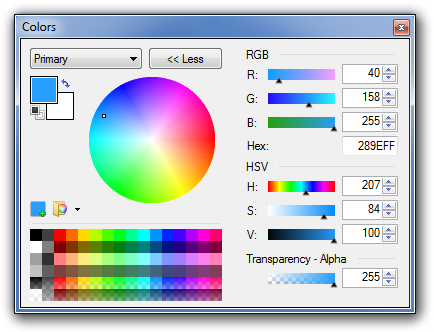
\includegraphics[height=170pt]{color.png}
\caption{选色}
\label{fig:colorwheel}
\end{figure}

CMYK模型认为纸张原本是白色或浅色背景的,在上面印刷某种颜料就会减少这种颜色光的反射,看上去就会是它的补色。印青色就会得到红色,印洋红得到绿,印黄得到蓝,青、洋红、黄三种颜色都印上就会得到黑色。彩色印刷有分色和套色过程,如果图形上有黑色直接拿黑颜料印刷会减少成本。CMYK中的字母K就代表key black。

在 \LaTeX 中,上述模型可以用不同的模式表示。比如RGB模型有三种模式:10进制的RGB模式,16进制的HTML模式,$[0,1]$实数的rgb模式。因为各种驱动支持不同的模式,用起来会很麻烦,\texttt{color} 宏包提供了驱动独立的使用界面。Uwe Kern\indexKern{} \footnote{1993年维尔茨堡大学 (University of Würzburg) 数学博士。} 的 \texttt{xcolor} 宏包更进一步,整合了12种色彩模式 (rgb, cmy, cmyk, hsb, Hsb, tHsb, gray, RGB, HTML, HSB, Gray, wave) ,提供了丰富的预定义颜色和命令。

\subsubsection{预定义和自定义颜色}

\texttt{xcolor} 宏包中预定义的颜色有:19种基本颜色,68种dvips颜色,151种SVG颜色,317种Unix/X11颜色。如要使用后三类颜色,引用宏包时需加相应预定义颜色集合选项:

\begin{Code}[]
\usepackage[dvipsnames]{xcolor}
\usepackage[svgnames]{xcolor}
\usepackage[x11names]{xcolor}
\end{Code}

如果这几百种预定义颜色还不能满足需要,可以使用 \verb|\definecolor| 命令自定义更多颜色。

\verb|语法: \definecolor{名称}{模式}{参数}|

\begin{example}[h]
\begin{Code}[]
\definecolor{myred}{RGB}{255,0,0}
\definecolor{mygreen}{HTML}{00FF00}
\definecolor{myblue}{rgb}{0,0,1}
\end{Code}
\caption{自定义颜色}
\label{exa:definecolor}
\end{example}

\subsubsection{彩色文字}

设置文字的颜色可以使用 \verb|\textcolor| 命令,\autoref{exa:textcolor} 中代码第2--4行和第5--7行输出效果相同。后三行的方法又称为抛弃型颜色定义法,因为只能用一次;事先定义了名字的话还可以重用。

\verb+语法: \textcolor{名称}|[模式]{代码}{文字}+

\begin{example}[h]
\LoadFBTDemo[numbers=left]{texlet/color-text}
\caption{彩色文字}
\label{exa:textcolor}
\end{example}

在当初电脑内存很宝贵的岁月里,引用 \texttt{xcolor} 宏包时不加预定义颜色集合选项就可以节省几十乃至几百个变量;当然这项节约对如今电脑的硬件配置不值一提,如果你坚持要做内存葛朗台,后三行的写法还是可以满足你变态的心理。

\subsubsection{彩色盒子}

\verb|\colorbox| 命令可以生成有彩色背景的盒子,它的语法和 \verb|\textcolor| 类似。\verb|\fcolorbox| 命令又给彩色盒子加了边框,它的第一个参数是边框的颜色。\autoref{exa:colorbox} 中使用了包老师喜欢的几种颜色,它们都来自 \texttt{svgnames}。

\begin{example}[h]
\begin{BTDemo}[numbers=left]
\colorbox{Lavender}{}
\colorbox{SkyBlue}{}
\colorbox{Wheat}{}
\fcolorbox{Silver}{Lavender}{}
\fcolorbox{RoyalBlue}{SkyBlue}{}
\fcolorbox{SandyBrown}{Wheat}{}
\end{BTDemo}
\caption{彩色盒子}
\label{exa:colorbox}
\end{example}

更多色彩功能可参考 \texttt{xcolor} 宏包的手册\citep{Kern_2007}。包老师敬告读者,在文档中要慎用彩色。包子曰:五音乱耳,五色炫目。

\subsection{绘图工具概览}
\label{sec:graph_tools}

与 \LaTeX 配套使用的矢量绘图工具中包老师较熟悉的有三种:\MP, PSTricks, PGF。限于篇幅和作者知识面,本文只对这三种工具作简单介绍。\MP, PSTricks, PGF的主要特点如下:

\begin{itemize}
\item 工作方式:\MP 离线绘图,生成的MPS (一种特殊的EPS) ;PSTricks和PGF都采用在线绘图的方式,也就是在 \LaTeX 文档内直接使用绘图命令。
\item 兼容性:\MP 生成的MPS需要先转为PDF才能被 \texttt{pdflatex}使用;PSTricks生成的EPS和 \texttt{pdflatex}不兼容;PGF提供针对各种驱动的接口,兼容性最好。
\item 功能:PSTricks有PostScript作后盾,功能最强;\MP{}擅长处理数学内容;PGF的流程图有独到之处。
\end{itemize}

后起之秀Asymptote颇有独到之处,英文读者可以参考其\href{http://asymptote.sourceforge.net/}{网站},中文读者可以参考milksea等人编写的\href{http://bbs.ctex.org/viewthread.php?tid=47893&extra=page%3D1}{文档}。

除了上述编程类工具,用户也可以考虑一些面向 \LaTeX 的绘图前端,比如Dia和Ipe,或者一些更通用的软件,比如gnuplot和Inkscape。

\bibliographystyle{unsrtnat}
\bibliography{lnotes2}
